% AdvanDEB Architecture Documentation
% This LaTeX document is intended for printable/PDF output.

\documentclass[11pt]{article}

\usepackage[margin=1in]{geometry}
\usepackage{hyperref}
\usepackage{graphicx}
\usepackage{enumitem}

\title{AdvanDEB System Architecture}
\author{AdvanDEB Project}
\date{\today}

\begin{document}

\maketitle

\section{Introduction}

This document provides a printable overview of the AdvanDEB system architecture. It summarizes the main components, external services, integration patterns, and core development environment.

The project consists of the following repositories:

\begin{itemize}[noitemsep]
  \item \texttt{advandeb-modeling-assistant} -- Main platform GUI (FastAPI + Vue) providing chat, knowledge exploration, and modeling features for all users.
  \item \texttt{advandeb-knowledge-builder} -- Toolkit/package for knowledge operations: fact extraction, document ingestion, graph building. No UI, imported by Modeling Assistant.
  \item \texttt{advandeb-MCP} -- Model Context Protocol server (Rust) exposing platform tools for LLM agent workflows.
  \item \texttt{advandeb-architecture} -- System-level documentation, diagrams, development log, and planning documents.
\end{itemize}

\section{Architecture Overview}

\textbf{advandeb-modeling-assistant} serves as the \textbf{main platform GUI} and single entry point for all users. It hosts authentication (Google OAuth), implements role-based access control, and provides the complete user interface including chat, knowledge exploration, document ingestion, and modeling scenarios.

\textbf{advandeb-knowledge-builder} is a \textbf{Python package/toolkit} (not a standalone application) providing robust operations for knowledge processing. It contains the logic for fact extraction, stylized facts generation, document ingestion pipelines, knowledge graph building, and review workflows. The Modeling Assistant imports this package and calls its functions as needed.

\textbf{advandeb-MCP} is a \textbf{tool server} that exposes platform operations as MCP tools for LLM agents. It wraps Knowledge Builder operations and provides LLM inference via Ollama. Used by Modeling Assistant for agent-powered features like chat and intelligent extraction.

\section{System Context}

Figure~\ref{fig:system-context} shows the high-level system context with the revised architecture model.

% Export system-context.puml to system-context.png before building
\begin{figure}[h]
  \centering
  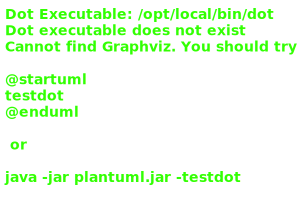
\includegraphics[width=0.9\textwidth]{../../diagrams/system-context.png}
  \caption{AdvanDEB System Context - Modeling Assistant as Main GUI}
  \label{fig:system-context}
\end{figure}

\section{Modeling Assistant (Main Platform GUI)}

The AdvanDEB Modeling Assistant is the \textbf{main platform interface} and single entry point for all users. It is a FastAPI + Vue application that provides:

\begin{itemize}[noitemsep]
  \item \textbf{Authentication}: Google OAuth integration and user management
  \item \textbf{Role-based Access}: Features shown/hidden based on user roles and capabilities
  \item \textbf{Chat Interface}: AI-powered chat using MCP server for LLM inference
  \item \textbf{Knowledge Exploration}: Browse facts, stylized facts, and knowledge graphs
  \item \textbf{Document Ingestion}: Interactive UI for uploading and processing documents
  \item \textbf{Modeling Features}: Scenario creation and model development
\end{itemize}

The Modeling Assistant backend imports the Knowledge Builder package to access knowledge operations, and calls the MCP server for agent-powered features.

Figure~\ref{fig:ma-container} shows the main containers and their relationships.

\begin{figure}[h]
  \centering
  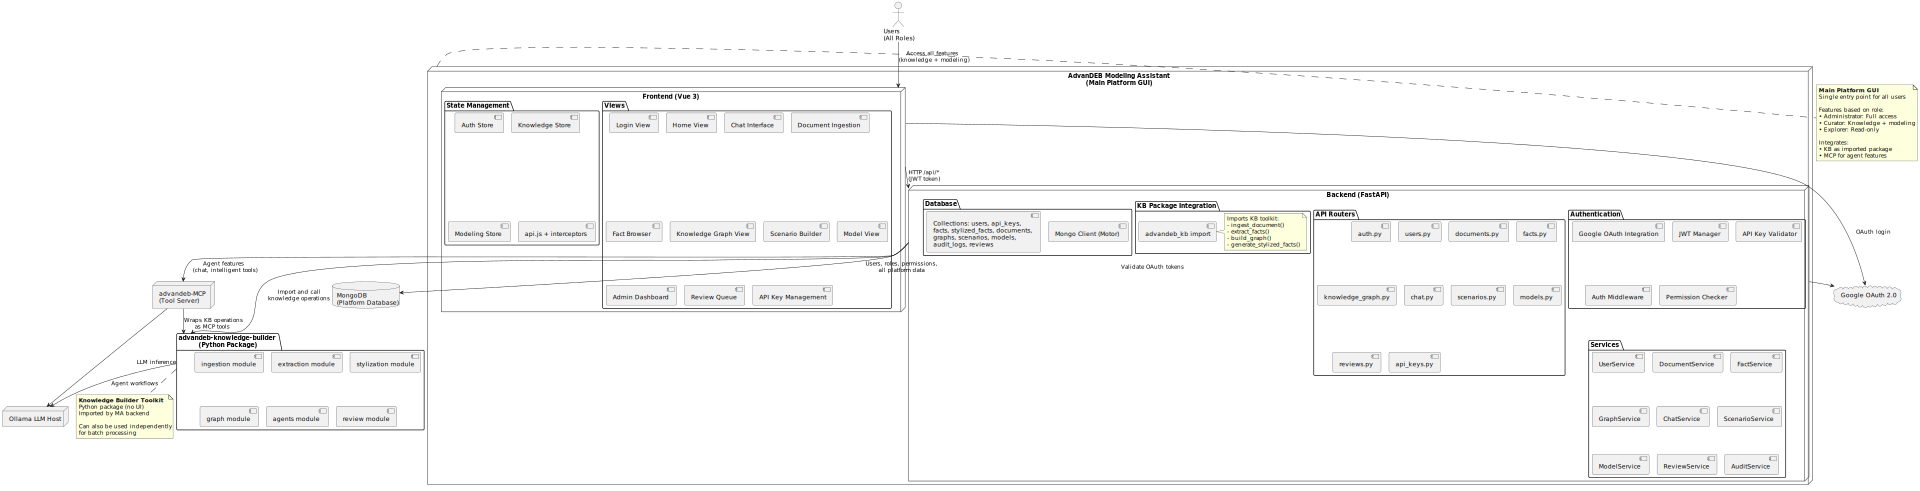
\includegraphics[width=0.9\textwidth]{../../diagrams/modeling-assistant-container.png}
  \caption{Modeling Assistant as Main GUI}
  \label{fig:ma-container}
\end{figure}

\section{Knowledge Builder (Toolkit/Package)}

The Knowledge Builder is a \textbf{Python package} (not a standalone application) that provides robust knowledge processing operations. It is imported by the Modeling Assistant backend.

\textbf{Key modules:}
\begin{itemize}[noitemsep]
  \item \texttt{ingestion} -- Document processing pipelines
  \item \texttt{extraction} -- Fact extraction algorithms
  \item \texttt{stylization} -- Stylized facts generation
  \item \texttt{graph} -- Knowledge graph building and querying
  \item \texttt{agents} -- Agent workflows with Ollama
  \item \texttt{review} -- Knowledge review and validation logic
\end{itemize}

The Knowledge Builder can also be used independently for batch processing operations outside of the web interface.

Figure~\ref{fig:kb-data-model} shows the conceptual data model for knowledge entities.

\begin{figure}[h]
  \centering
  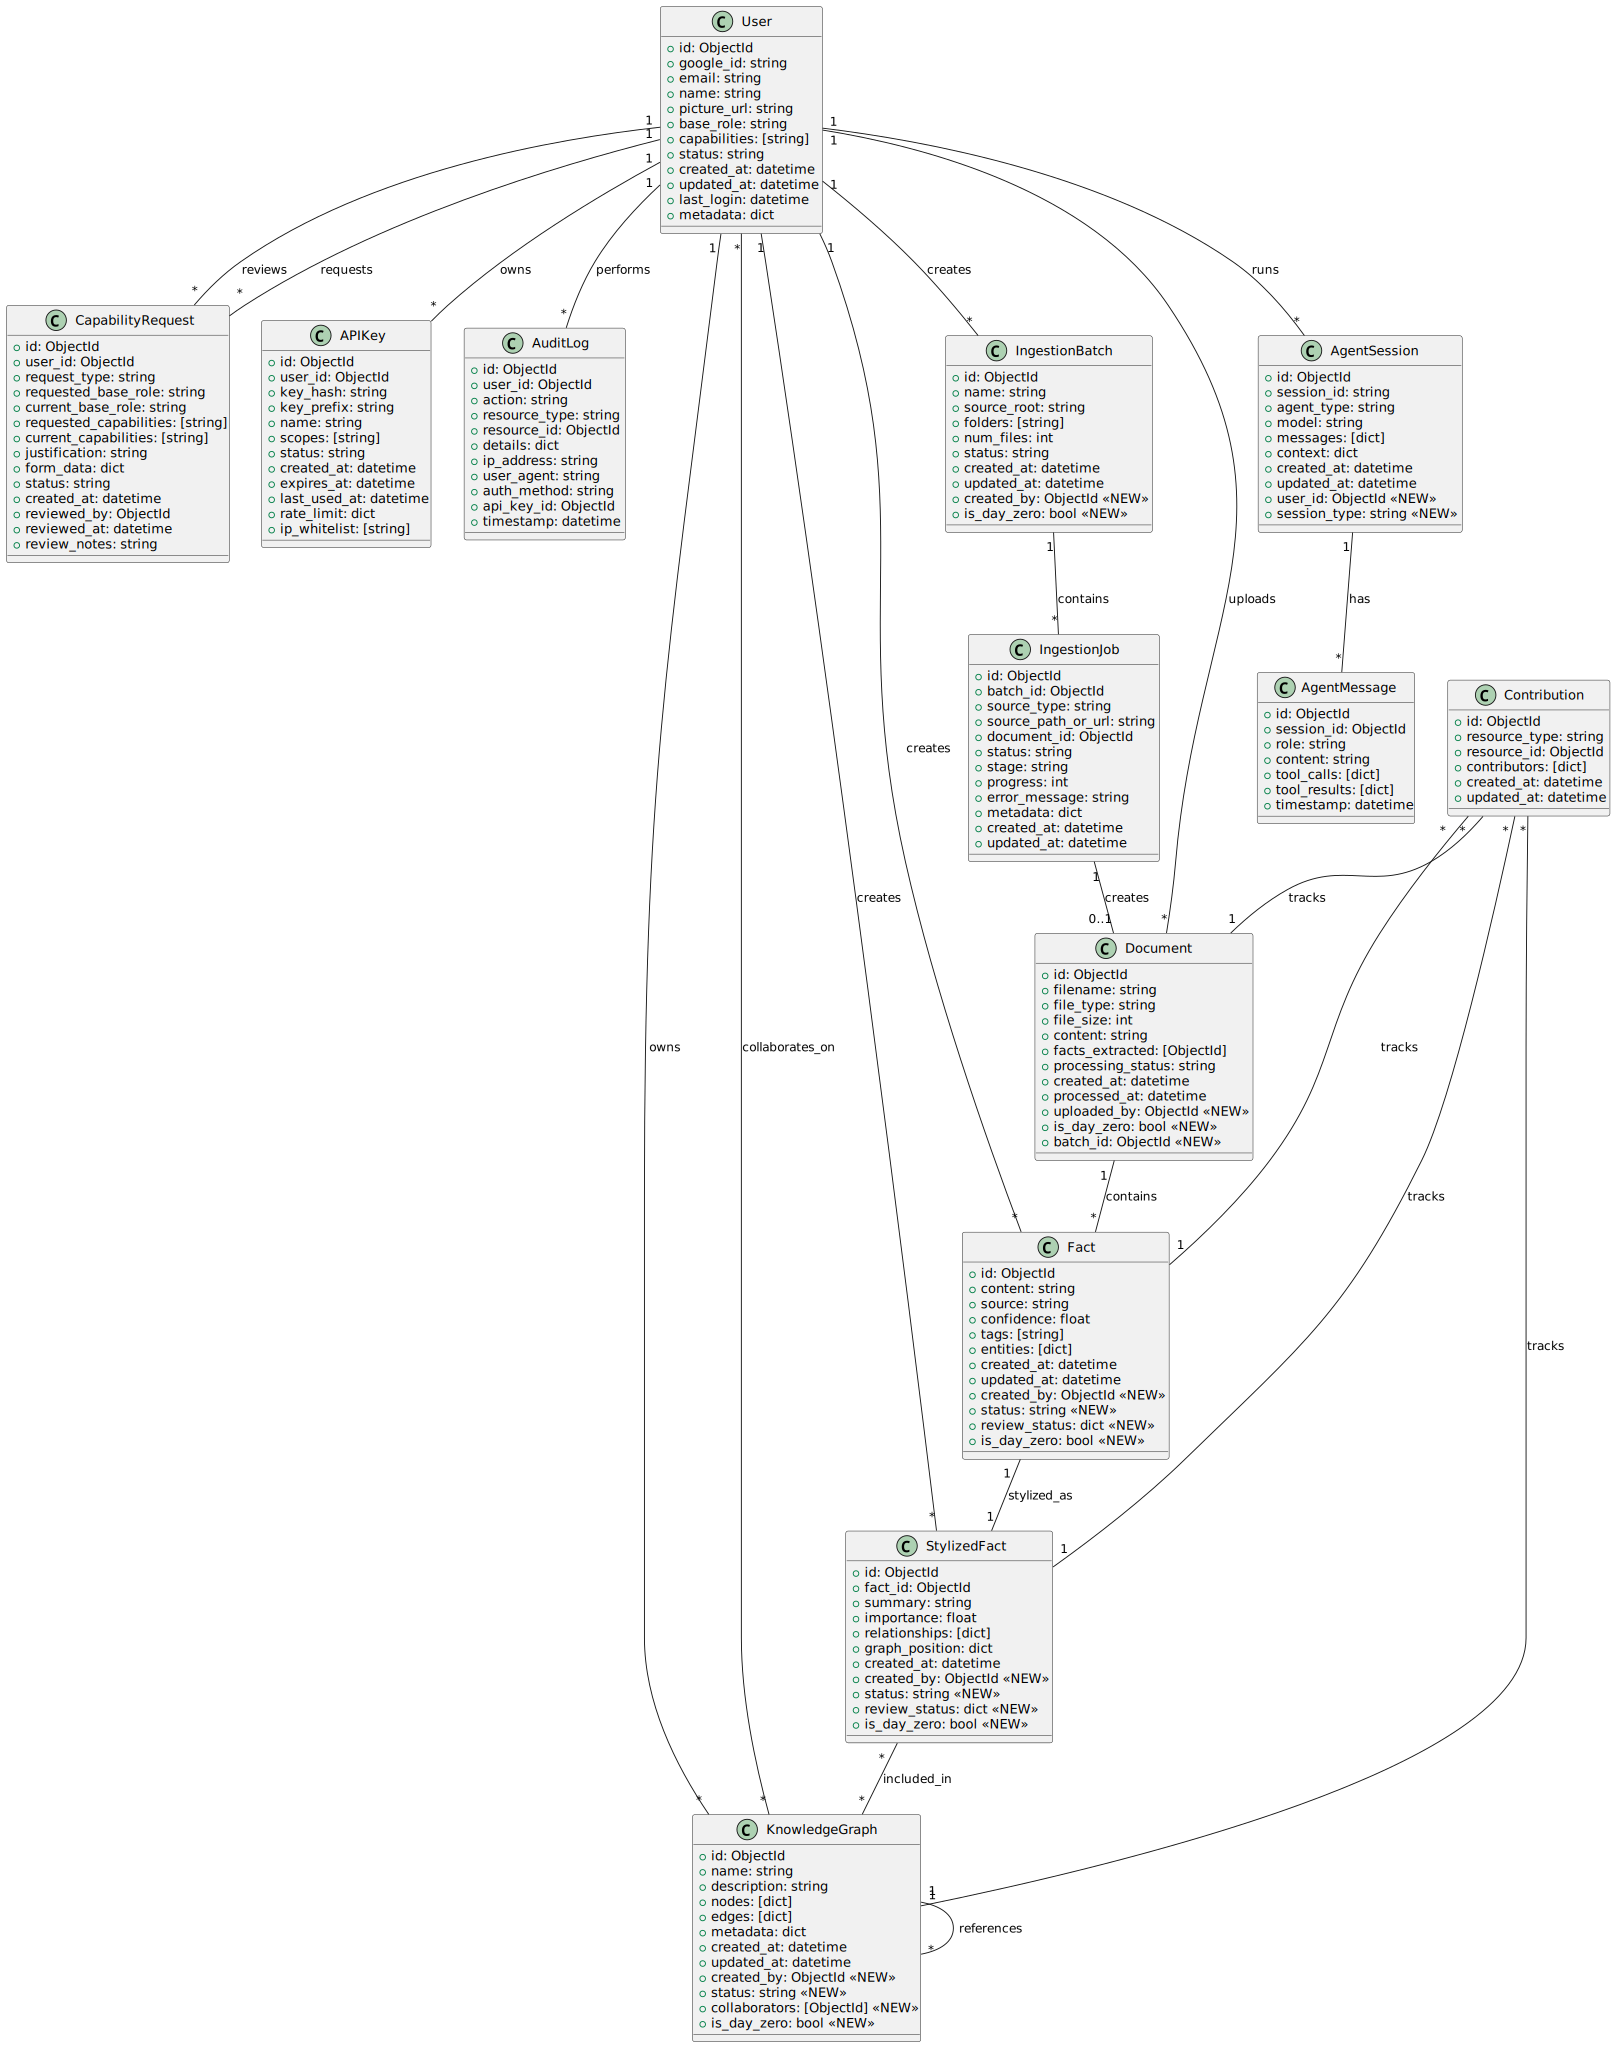
\includegraphics[width=0.9\textwidth]{../../diagrams/knowledge-builder-data-model.png}
  \caption{Knowledge Builder Conceptual Data Model}
  \label{fig:kb-data-model}
\end{figure}

\subsection{Document Ingestion Flow}

When a user uploads a document through the Modeling Assistant GUI, the MA backend calls Knowledge Builder package functions to process it.

The document ingestion and fact extraction sequence is illustrated in Figure~\ref{fig:doc-ingestion}.

\begin{figure}[h]
  \centering
  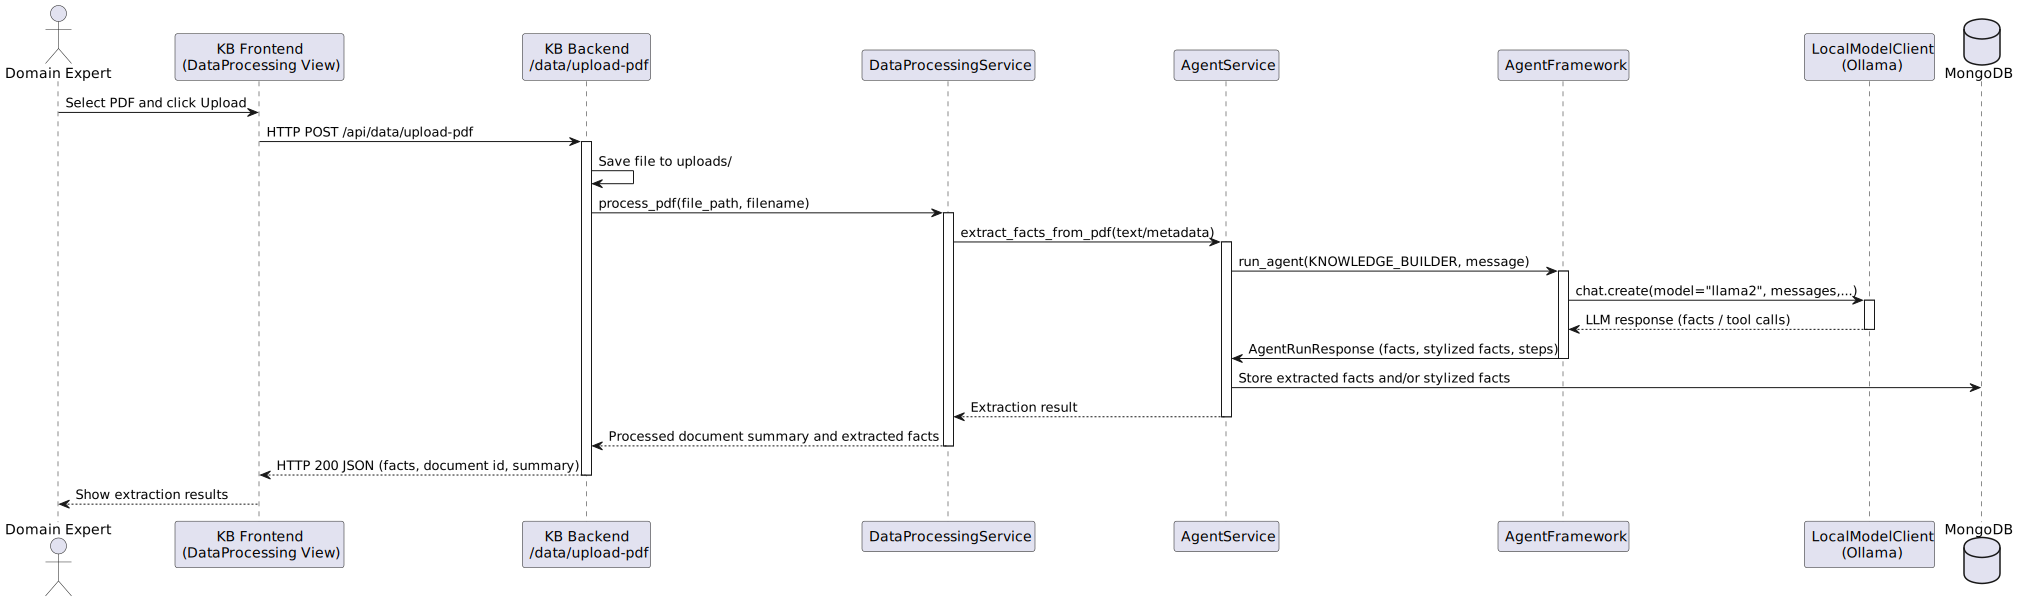
\includegraphics[width=0.9\textwidth]{../../diagrams/document-ingestion-sequence.png}
  \caption{Document Ingestion and Fact Extraction}
  \label{fig:doc-ingestion}
\end{figure}

\section{MCP Server (Tool Server)}

The advandeb-MCP server is an internal service that exposes platform operations as MCP tools for LLM agent workflows.

\textbf{Key Features:}
\begin{itemize}[noitemsep]
  \item Wraps Knowledge Builder operations as MCP tools
  \item Provides LLM inference via Ollama
  \item Internal service (no authentication required)
  \item Used by Modeling Assistant for chat and agent features
  \item Rust-based for high performance
\end{itemize}

\textbf{Tool Categories:}
\begin{itemize}[noitemsep]
  \item Knowledge Building Tools: fact extraction, document ingestion, stylized facts
  \item Knowledge Query Tools: search facts, graph traversal
  \item Modeling Tools: scenario analysis, parameter suggestions
  \item Chat Tools: conversational LLM interface with knowledge context
\end{itemize}

\section{Development Environment}

All services use a single Conda environment named \texttt{advandeb}. The canonical \texttt{environment.yml} is stored in the \texttt{advandeb-architecture} repository.

To create and activate the environment:

\begin{verbatim}
conda env create -f environment.yml
conda activate advandeb
\end{verbatim}

Core external services:

\begin{itemize}[noitemsep]
  \item MongoDB (default: \texttt{mongodb://localhost:27017})
  \item Ollama (default: \texttt{http://localhost:11434})
\end{itemize}

\section{Integration Architecture}

The platform uses a simple integration model:

\begin{itemize}[noitemsep]
  \item \textbf{Modeling Assistant} imports \textbf{Knowledge Builder} as a Python package
  \item \textbf{Modeling Assistant} calls \textbf{MCP Server} via internal HTTP/WebSocket
  \item \textbf{MCP Server} wraps \textbf{Knowledge Builder} operations as MCP tools
  \item All components share the same \textbf{MongoDB} database
\end{itemize}

\subsection{Data Flow Examples}

\textbf{Example 1: Document Upload}
\begin{enumerate}[noitemsep]
  \item User logs into Modeling Assistant GUI
  \item User uploads PDF via web interface
  \item MA backend imports KB package: \texttt{from advandeb\_kb import ingest\_document}
  \item KB package processes document and stores in MongoDB
  \item MA returns success response to frontend
\end{enumerate}

\textbf{Example 2: AI Chat}
\begin{enumerate}[noitemsep]
  \item User opens chat interface in MA
  \item User types question
  \item MA backend sends request to MCP server
  \item MCP invokes tools (using KB functions) and calls Ollama
  \item MCP returns formatted response
  \item MA displays chat response to user
\end{enumerate}

\subsection{Authentication and Authorization}

All authentication is handled by the Modeling Assistant:
\begin{itemize}[noitemsep]
  \item Google OAuth 2.0 integration
  \item JWT tokens for API authentication
  \item Role-based access control (Administrator, Curator, Explorer)
  \item Capability-based permissions (Agent Access, Analytics, Reviewer)
\end{itemize}

The Knowledge Builder package and MCP server operate as internal services without authentication. User attribution is maintained by MA before calling these services.

\section{Future Work}

Planned extensions to this architecture and documentation include:

\begin{itemize}[noitemsep]
  \item Complete implementation of Modeling Assistant as main GUI platform
  \item Refactoring Knowledge Builder into Python package structure
  \item MCP server tool implementations for KB and MA operations
  \item Enhanced role-based access control and capability management
  \item Additional visualization tools for knowledge graphs
  \item Batch processing workflows using KB package independently
  \item Performance optimization for large-scale knowledge bases
\end{itemize}

\section{References}

For more detailed information, consult:

\begin{itemize}[noitemsep]
  \item \texttt{SYSTEM-OVERVIEW.md} -- Comprehensive system architecture
  \item \texttt{ARCHITECTURE-REVISION.md} -- Detailed explanation of architectural model
  \item \texttt{MCP-PLAN.md} -- MCP server implementation plan
  \item \texttt{ROADMAP.md} -- Development timeline and phases
  \item \texttt{USER-MANAGEMENT-PLAN.md} -- Authentication and authorization details
\end{itemize}

\end{document}
